%% tags: curves, plot, curve, plots, axis, edgeLabel, edgeLabels, intersections
\PassOptionsToPackage{usenames,dvipsnames}{xcolor}
\documentclass[tikz,border=2]{standalone}
\usetikzlibrary{intersections,shadows,arrows,shapes,positioning,calc,backgrounds,fit}
%%
\definecolor{Green}{HTML}{66C2A5}
\definecolor{Blue}{HTML}{8DA0CB}
\definecolor{Orange}{HTML}{FC8D62}
%%
\makeatletter
\newcommand{\gettikzxy}[3]{%
\tikz@scan@one@point\pgfutil@firstofone#1\relax
\edef#2{\the\pgf@x}%
\edef#3{\the\pgf@y}%
}
\makeatother
% Define the layers to draw the diagram
\begin{document}
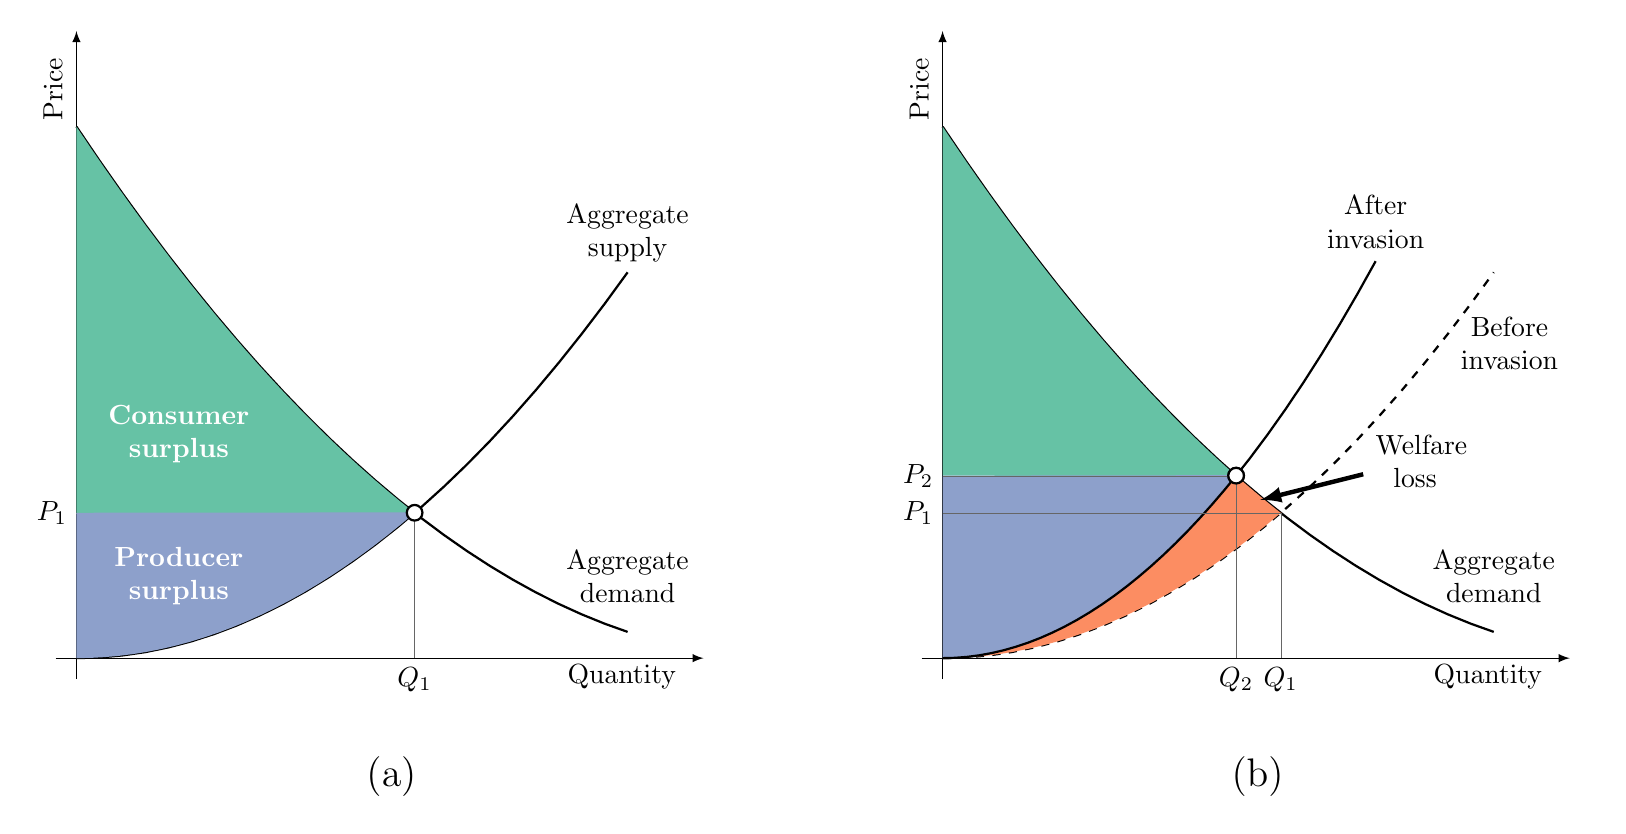
\begin{tikzpicture}
[node distance=1cm,scale=1,
axis/.style={thin,inner sep=2pt,>=latex, shorten >=1pt, shorten <=1pt},
curve/.style={thick},
point/.style={circle,inner sep=2pt,fill=white,draw=black,thick},
ref/.style={ultra thin,black!60,text=black},
lbl/.style={font=\bfseries,white}
]
\newcommand{\supplycurve}{\x,{((\x)^2)/10 +0}}
\newcommand{\supplycurvenew}{\x,{((\x)^2)/6 +0}}
\newcommand{\demandcurve}{\x,{((\x-9)^2)/12}}
\begin{scope}
%% axes
\node (origin) at (0,0) {};
\draw[axis,->,name path=xaxis] (-.3,0) -- (8,0) node[near end,below,shift={(1,0)}] {Quantity};
\draw[axis,->,name path=yaxis] (0,-.3) -- (0,8) node[rotate=90,near
end,above,shift={(1.3,0.1)}] {Price};
%% supply
\draw[curve,name path=supply] plot [domain=0:7] (\supplycurve) 
node[shift={(0,.5)}] {\parbox{2cm}{\centering Aggregate supply}};
%% demand
\draw[curve,name path=demand] plot [domain=0:7] (\demandcurve)
node[shift={(0,.7)}] {\parbox{2cm}{\centering Aggregate demand}};
%% intersections
\path[name intersections={of=supply and demand,by=equilibrium}];
\path[name intersections={of=yaxis and demand,by=yDemand}];
\path[name intersections={of=yaxis and supply,by=ySupply}];
%% equilibrium
\node at (equilibrium) {};
\draw[ref] (equilibrium |- origin) node[below]{$Q_1$} |- (equilibrium -|
origin) node[left]{$P_1$};
%% consumer surplus
%%%% extract x coordinate of (equilibrium)
\newdimen{\ex}
\gettikzxy{(equilibrium)}{\tx}{\ty};
\pgfmathsetmacro\ex{\tx/28.4}
%%
\fill[Green,opacity=1] (yDemand) --
plot[domain=0:\ex] (\demandcurve) -- (equilibrium -| origin) -- cycle;
\node[lbl,shift={(1.3,1)}] at (equilibrium -| origin)
{\parbox{2cm}{\centering Consumer surplus}};
\fill[Blue,opacity=1] (ySupply) -- 
plot[domain=0:\ex] (\supplycurve) -- (equilibrium -| origin) -- cycle;
\node[lbl,shift={(1.3,-.8)}] at (equilibrium -| origin)
{\parbox{2cm}{\centering Producer surplus}};
\node[point] at (equilibrium) {};
\node[font=\Large] at (4,-1.5) {(a)};
%%
\end{scope}
%%
\begin{scope}[shift={(11,0)}]
%% axes
\node (origin) at (0,0) {};
\draw[axis,->,name path=xaxis] (-.3,0) -- (8,0) node[near end,below,shift={(1,0)}] {Quantity};
\draw[axis,->,name path=yaxis] (0,-.3) -- (0,8) node[rotate=90,near
end,above,shift={(1.3,0.1)}] {Price};
%% supply before invasion
\draw[curve,name path=supplyOld,dashed] plot [domain=0:7] (\supplycurve) 
node[shift={(0.2,-.9)}] {\parbox{2cm}{\centering Before invasion}};
%% supply after invasion
\draw[curve,name path=supplyNew] plot [domain=0:5.5] (\supplycurvenew) 
node[shift={(0,.5)}] {\parbox{2cm}{\centering After invasion}};
%% demand
\draw[curve,name path=demand] plot [domain=0:7] (\demandcurve)
node[shift={(0,.7)}] {\parbox{2cm}{\centering Aggregate demand}};
%% intersections
\path[name intersections={of=supplyOld and demand,by=equilibriumOld}];
\path[name intersections={of=supplyNew and demand,by=equilibriumNew}];
\path[name intersections={of=yaxis and demand,by=yDemand}];
\path[name intersections={of=yaxis and supplyNew,by=ySupply}];
%% consumer surplus
%%%% extract x coordinate of (equilibriumNew)
\newdimen{\exOld}
\gettikzxy{(equilibriumOld)}{\tx}{\ty};
\pgfmathsetmacro\exOld{\tx/28.4}
%%
\newdimen{\exNew}
\gettikzxy{(equilibriumNew)}{\tx}{\ty};
\pgfmathsetmacro\exNew{\tx/28.4}
%%
\fill[Green,opacity=1] (yDemand) --
plot[domain=0:\exNew] (\demandcurve) -- (equilibriumNew -| origin) -- cycle;
\fill[Blue,opacity=1] (ySupply) -- 
plot[domain=0:\exNew] (\supplycurvenew) -- (equilibriumNew -| origin) -- cycle;
\node[point] at (equilibriumNew) {};
%%
\fill[Orange,opacity=1] (equilibriumNew) -- 
plot[domain=\exNew:\exOld] (\demandcurve) -- 
plot[domain=\exOld:0] (\supplycurve) -- 
plot[domain=0:\exNew] (\supplycurvenew) -- cycle;
\draw[curve] plot[domain=0:\exNew] (\supplycurvenew); % for curve to be visible
%%
%% equilibriums
\node at (equilibriumNew) {};
\draw[ref] (equilibriumNew |- origin) node[below]{$Q_2$} |- (equilibriumNew -|
origin) node[left]{$P_2$};
%%%%
\node at (equilibriumOld) {};
\draw[ref] (equilibriumOld |- origin) node[below]{$Q_1$} |- (equilibriumOld -|
origin) node[left]{$P_1$};
%%
\node (wl) at (6,2.5) {\parbox{1cm}{\centering Welfare loss}};
\draw[axis,ultra thick,->] (wl) -- +(-2,-.5);
%%
\node[point] at (equilibriumNew) {};
\node[font=\Large] at (4,-1.5) {(b)};
\end{scope}
\end{tikzpicture}
\end{document}

